\title{\Large ES2A EEP-02  \\[0.5cm]
        \bf\Large Vaccine strategies}
\author{\large Florent Pollet \ \\}
\date{\large\today}

\makeatletter
    \begin{titlepage}
        \begin{center}
	   { 
\includegraphics[width=12cm]{imgs/mp_logo.png}}
	   {\ \\ \ \\}
        \vbox{}\vspace{2cm}
            {\@title }\\[1cm] 
            %{ \includegraphics[width=7cm]{imgs/cover.PNG}}\\[1cm]
            {\@author}

            {\large \ \\ Supervisor: \bf Véronique Stoven\\ \ \\}
            {\@date\\}

        \end{center}

        \vspace{4cm}
        \begin{figure}[H]
            \centering
            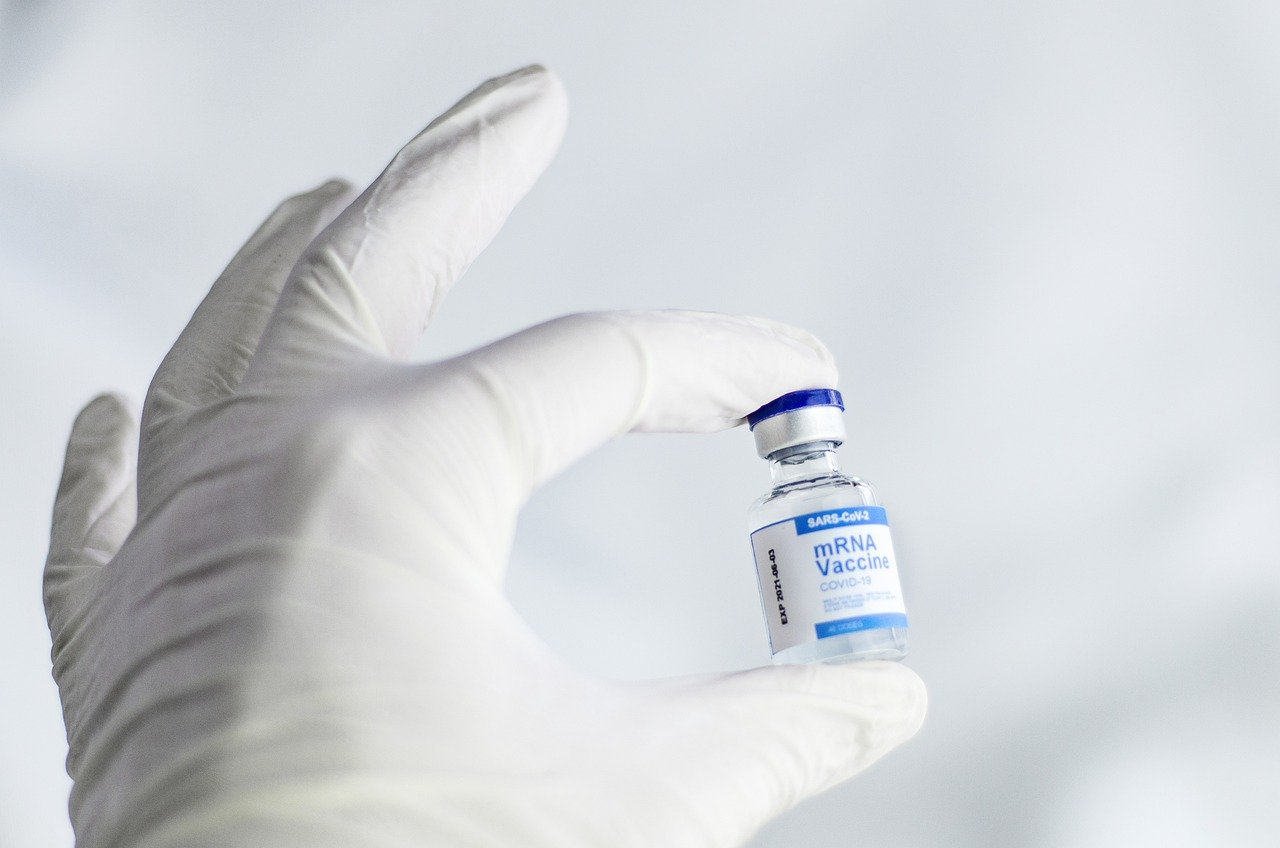
\includegraphics[width=0.4\textwidth]{imgs/vaccineCover.jpg}
        \end{figure}

    \end{titlepage}


    \begin{abstract}        
        In a context of a pandemic and major doubts towards vaccination among populations, this paper deals with vaccine strategies, especially how mRNA vaccines are revolutionizing them.
        It is clear that immunology represents a complex field of science,
            and nowadays the breakthroughs in biotechnologies are offering new possibilities to accelerate vaccine development, efficiency and safety as well as a better understanding
            our immune system.
        This paper aims at summarizing the different vaccine techniques with a special attention to mRNA vaccines\footnote{Messenger RiboNucleic Acid}, in order to
            have an overview of the current vaccine strategies which are going to evolve.
        % implications, finding, methods ? go further ?
    \end{abstract}

        
    \begin{remerciements}
        I cannot express enough thanks to my teacher Véronique Stoven for her interesting lessons about molecular and synthetic biology,
            which inspired me this topic as well as for her help in the writing of this article.
        I absolutely loved doing research and writing this report.
    \end{remerciements}


    \tableofcontents


    \newpage

    \makeatother